\documentclass{fpgairpods}
\usepackage[letterpaper, margin=1in]{geometry}

\addbibresource{report.bib}
\graphicspath{{figs/}}

\setlist{noitemsep, topsep=0pt}

\begin{document}

\title{\textit{FPGAirPods}: Implementing Active Noise Cancellation on a Xilinx Nexys7 FPGA}
\date{\textit{Massachusetts Institute of Technology} \\ \today}
\author{Ben Kettle \\ \ttt{bkettle@mit.edu} 
\and Nicholas Ramirez \\ \ttt{ramirezn@mit.edu} \and Gokul Kolady \\ \ttt{gokulk@mit.edu}}

\maketitle
\tableofcontents

\newpage
\begin{multicols}{2}
\section{Introduction}

	Noise cancellation is in demand. At the time of writing this, Apple has just released AirPods Max for \$550.

\section{Overview}
Our 6.111 final project aims to implement active noise cancellation as seen in over-ear and in-ear headphones such as the Bose QC35 and the AirPods Pro (hence the name). In order to do this, we will first need to create a physical model of a single headphone (one ear cup) that we will use to test. Inside the ear cup, we will install a speaker (far from the ear) and a digital microphone (closer to the ear). We will also use a digital microphone external to the ear cup in order to capture ambient noise.

The FPGA itself will handle the computational side of the active noise cancellation. This will primarily involve an adaptive filter that will continually improve its coefficients in order to minimize the error function --- i.e., the noise that makes it through and is not cancelled out. We run the input from the external microphone through this filter, and play the filtered result out of the speaker with the aim of cancelling noise.


\end{multicols}



\begin{figure}
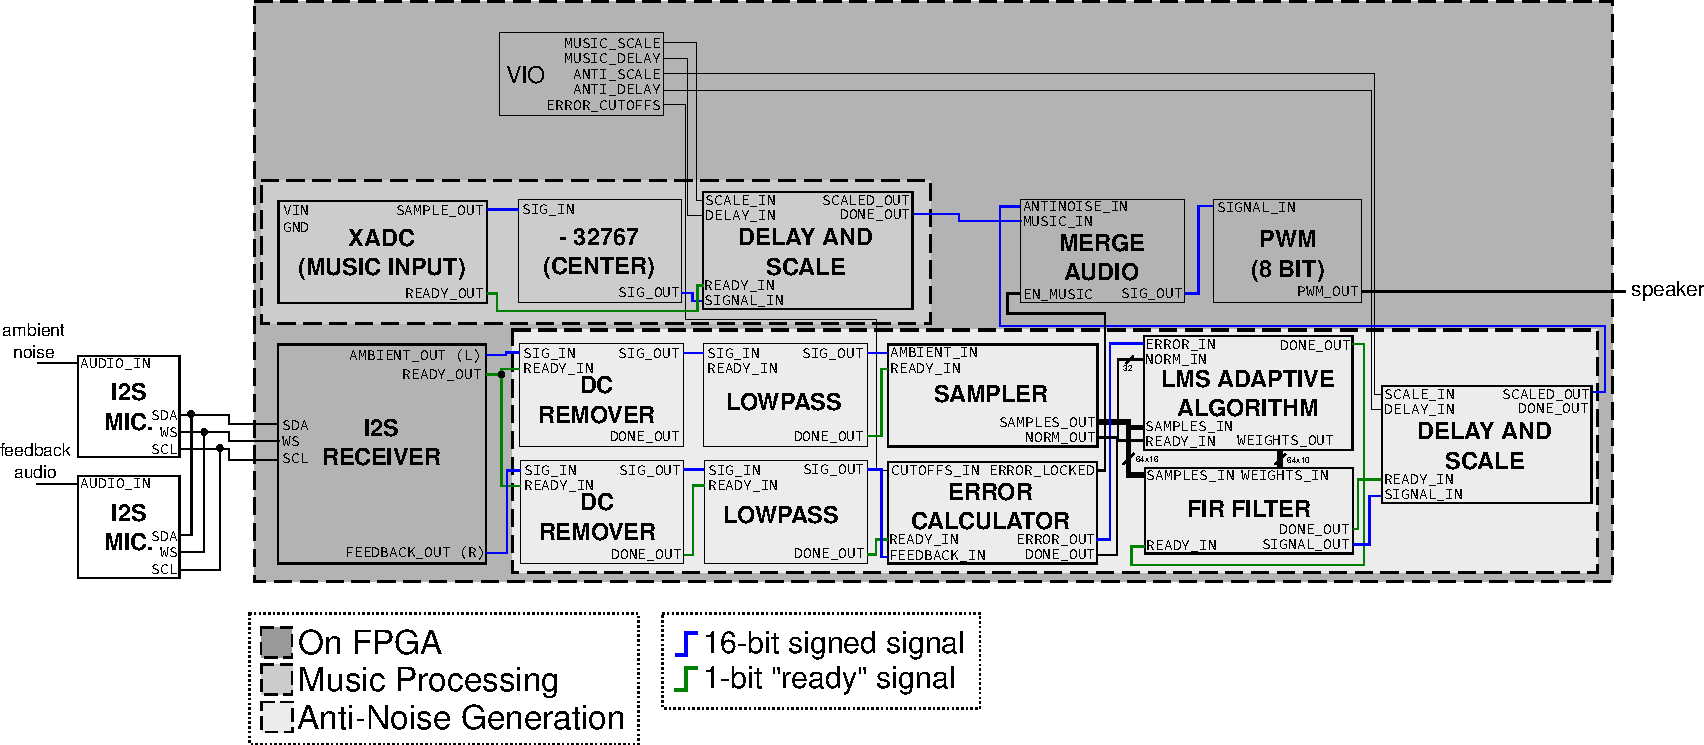
\includegraphics[width=\textwidth]{./figs/block_diagram.pdf}
\caption{The high-level block diagram for our system.}
\label{fig:blockdiagram}
\end{figure}


\newpage
\section{Hardware Testing Setup (Ben)}
\subsection{Testing Hardware (Ben)}
In order to demonstrate that our system was functional, a system to test on was crucial. This system would include the FPGA as a processing center with a variety of peripherals.

\begin{figure}[h]
\centering
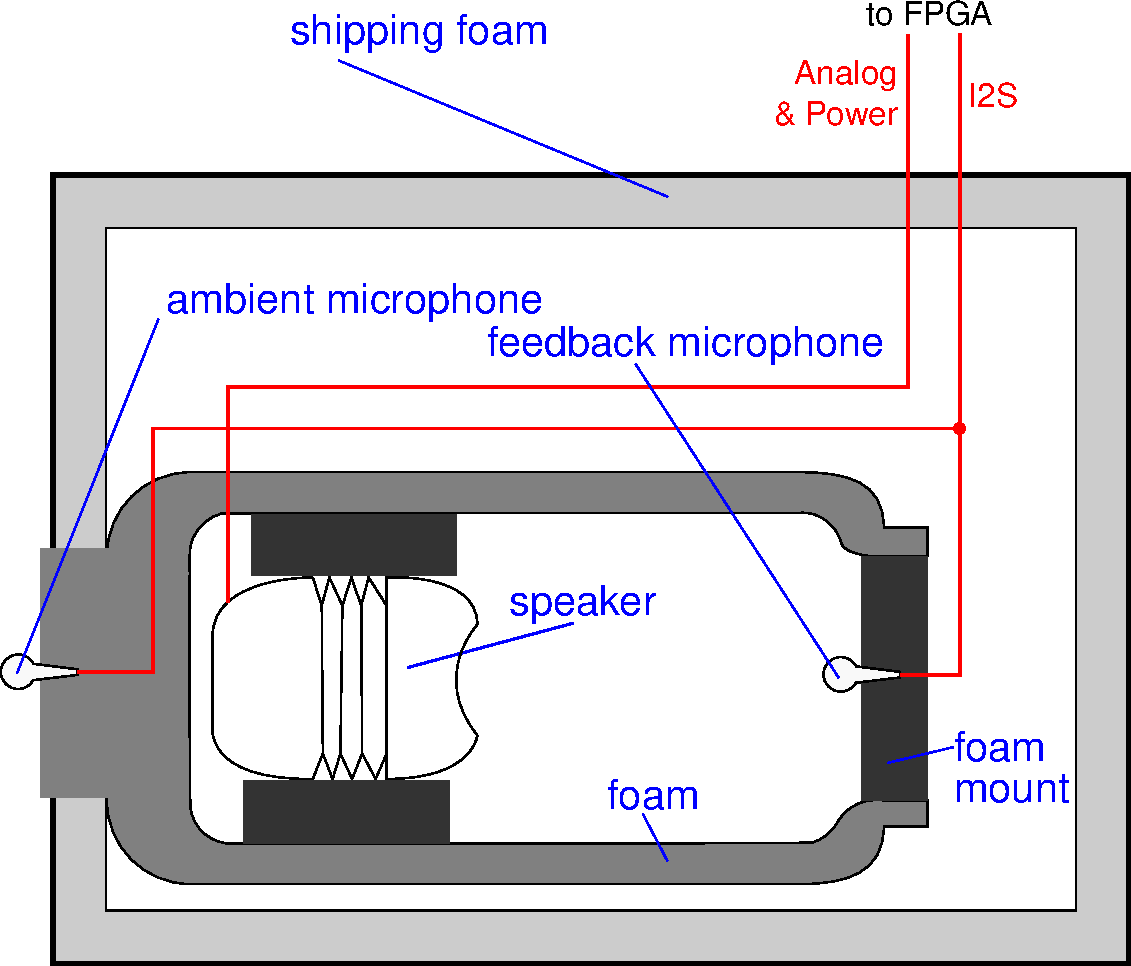
\includegraphics[width=300pt]{./figs/system_diagram_with_text.pdf}
\caption{The peripherals that will be included in our project}
\label{fig:peripherals}
\end{figure}

\section{Implementation Details}
Our implementation was structured as a series of modules each applying some processing on the incoming ambient noise signal. We devised a common scheme for all these modules to share, where in addition to any other samples or signals it requires, each module includes a \ttt{ready_in} signal and outputs a \ttt{ready_out} signal---each 1 clock cycle long. This allows us to chain many of these modules together, feeding \ttt{done_out} of each into \ttt{ready_in} of the next.

\subsection{I2S Receiver (Ben)}
This module is the origin of the \ttt{ready_in} pulse chain described above---it implements the I2S protocol as described in the datasheet for the microphones we use\autocite{mic_datasheet}. In essence, this requires the creation of an \ttt{LRCLK} signal that controls whether the left (ambient) or right (feedback) mic will currently transmit. For every change of this clock, the corresponding microphone would begin sending a new sample. We drove this clock at the 4MHz, the maximum rate tolerated by the microphones, for a sampling rate through our system of 65 kHz.

\subsection{FIR Filter - \textit{Niko}}
The FIR Filter module convolves the external ambient noise with a set of filter coefficients in order to produce an anti-noise signal. This anti-noise signal is later used to cancel out the ambient noise that makes it into the ear cup. These coefficients are set continuously by the LMS adaptive algorithm module.
\subsubsection{Inputs}
\begin{itemize}
    \item \ttt{external_signal_in[15:0]}: The current sample from the external microphone that will be filtered.
    \item \ttt{weights_in[31:0][9:0]}: Coefficients that the filter will use for convolution.
\end{itemize}
\subsubsection{Outputs}
\begin{itemize}
    \item \ttt{antinoise_out[15:0]}: Anti-noise signal that will be used to cancel out ambient noise.
\end{itemize}
\subsubsection{Complexity/Level of Performance}
This module will be time sensitive, as we will want to calculate the output corresponding to a given input in very little time in order to enable effective noise cancellation. Because of this, we anticipate a significant amount of time to be spent streamlining the functionality of the filter module and improving its performance. As part of this, we need fast access to the previous samples to use for the convolution, so these previous samples from the external microphone will be stored in a circular buffer as a 32 element array with each element 16 bits wide. Implementing this as a BRAM would be to slow, so it will be implemented with distributed RAM. Some optimization that we are considering for this module is performing the additions in a tree structure rather than sequentially and streamlining the multiplications if necessary. We expect this to include 32 multiplications and 32 additions.

\subsubsection{Testing - \textit{Gokul}}
Testing for this module will consist of simple inputs similar to those seen in Lab 5a with known filter coefficients, such as a low pass filter with an impulse input, a sine input, etc. If these show the results that we expect, we can conclude that the FIR filter works. Later, we will also test it in conjunction with the LMS.

\subsection{LMS \& NLMS Adaptive Algs. - \textit{Gokul \& Niko}}
This module uses the LMS adaptive algorithm in order to update the coefficients of the FIR Filter for better noise cancellation. This algorithm takes advantage of the steepest descent optimization method, which analyzes the impact of the previous filter coefficients on the observed error and computes appropriate adjustments. This update is accomplished using the following equation\cite{lmsfilter}, where $b_k(n)$ is the FIR coefficient for a given $k$ value and a given timestep $n$, $\Lambda$ is a predefined step size or learning rate that defines how quickly the filter weights change, $e(n)$ is the calculated error, $f(n)$ is the value of the noise sample from the external microphone at a timestep $n$, and $M$ is the number of coefficients in the FIR filter:
\[ b_k(n + 1) = b_k(n) + \Lambda e(n)f(n-k) \]
\[ k = 0, 1, 2,\ldots,  M-1 \]

\subsubsection{Inputs}
\begin{itemize}
    \item \ttt{external_signal_in[15:0]}: The current sample from the external microphone (previous samples get used in weight update formula, so they must be stored in this module).
    \item \ttt{error_in[15:0]}: The error between the internal microphone signal and the desired signal.
\end{itemize}
\subsubsection{Outputs}
\begin{itemize}
    \item \ttt{weights_out[31:0][9:0]}: Updated coefficients to be used by the FIR filter in the next timestep for improved anti-noise generation.
\end{itemize}
\subsubsection{Complexity/Level of Performance}
To implement this operation, we will need to store the last $M$ noise inputs from the external microphone along with the full last set of filter coefficients. Previous samples from the external microphone will be stored in a circular buffer as a 32 element array each 16 bits wide, and the coefficients will be stored similarly in distributed RAM if possible, 32 elements each 10 bits wide.

\subsubsection{Testing - \textit{Niko}}
Testing this module will be a bit more involved than some of the others due to its not well-defined behavior, but in order to test the behavior we will need to have a working FIR module. With this module in place, we can then test the ability of the LMS algorithm to recreate the coefficients of a given filter. In other words, we can have our "desired" signal be the result of passing some input through an arbitrary filter, use this desired signal to calculate the error $e(n)$, and pass this error into our LMS module. If the input of the LMS module is the same as the input to this mystery filter, we can conclude that the LMS algorithm is functioning as necessary.

\subsection{Error Calculator - \textit{Gokul}}
The error calculator module monitors the error our system encounters in order to pass it into the NLMS.

\subsubsection{Inputs}
\begin{itemize}
    \item \ttt{antinoise_in[15:0]}: One of the two signals to be added.
    \item \ttt{music_signal_in[15:0]}: The other signal to be added.
\end{itemize}
\subsubsection{Outputs}
\begin{itemize}
    \item \ttt{full_digital_signal_out[15:0]}: The sum of the two signals.
\end{itemize}

\subsection{DC Remover (Gokul)}
removes dc

\subsection{Music Receiver (Ben)}
receives music

\subsection{Audio Mixing (Ben)}
mixes audio

\section{Challenges}
This project had many challenges.

\section{Reflections}

\section{References}

\printbibliography

\end{document}
